%% ----------------------------------------------------------------
%% Thesis.tex -- MAIN FILE (the one that you compile with LaTeX)
%% ---------------------------------------------------------------- 

% Set up the document
\documentclass[a4paper, 11pt, oneside]{Thesis}  % Use the "Thesis" style, based on the ECS Thesis style by Steve Gunn

% Include any extra LaTeX packages required
\usepackage[square, numbers, comma, sort&compress]{natbib}  % Use the "Natbib" style for the references in the Bibliography
\usepackage[nottoc]{tocbibind} % bind bibliography to the table of contents
\usepackage{verbatim}  % Needed for the "comment" environment to make LaTeX comments
\usepackage{vector}  % Allows "\bvec{}" and "\buvec{}" for "blackboard" style bold vectors in maths
\usepackage[table]{xcolor}
\hypersetup{urlcolor=black, colorlinks=true}  % Colours hyperlinks in black, can be distracting if there are many links and colored blue.
\usepackage{graphicx}
\usepackage{subcaption}
\usepackage{wrapfig}
\usepackage[utf8]{inputenc}
\usepackage[export]{adjustbox}
\usepackage{array}
\usepackage[table]{xcolor}
\setlength{\arrayrulewidth}{1mm}
\setlength{\tabcolsep}{18pt}
\graphicspath{{Figures/}}  % Location of the graphics files (set up for graphics to be in PDF format)

%% ----------------------------------------------------------------
\begin{document}
\frontmatter      % Begin Roman style (i, ii, iii, iv...) page numbering

% Set up the Title Page
\title  {Edge/Fog Computing - Containerization on Single Board Computers }
\authors  {Jodie Bermingham}
            
\addresses  {\groupname\\\deptname\\\univname}  % Do not change this here, instead these must be set in the "Thesis.cls" file, please look through it instead
\date       {\today}
\subject    {}
\keywords   {}

\maketitle
%% ----------------------------------------------------------------

\setstretch{1.3}  % It is better to have smaller font and larger line spacing than the other way round

% Define the page headers using the FancyHdr package and set up for one-sided printing
\fancyhead{}  % Clears all page headers and footers
\rhead{\thepage}  % Sets the right side header to show the page number
\lhead{}  % Clears the left side page header

\pagestyle{fancy}  % Finally, use the "fancy" page style to implement the FancyHdr headers

%% ----------------------------------------------------------------
% Declaration Page required for the Thesis
\Declaration{

\addtocontents{toc}{\vspace{1em}}  % Add a gap in the Contents, for aesthetics

I, Jodie Bermingham , declare that this thesis titled, 'Migrating Micro-Services between Single Board Computers using Containerization' and the work presented in it are my own. I confirm that:

\begin{itemize} 
\item[\tiny{$\blacksquare$}] This work was done wholly or mainly while in candidature for an undergraduate degree at Cork Institute of Technology.
 
\item[\tiny{$\blacksquare$}] Where any part of this thesis has previously been submitted for a degree or any other qualification at Cork Institute of Technology or any other institution, this has been clearly stated.
 
\item[\tiny{$\blacksquare$}] Where I have consulted the published work of others, this is always clearly attributed.
 
\item[\tiny{$\blacksquare$}] Where I have quoted from the work of others, the source is always given. With the exception of such quotations, this project report is entirely my own work.
 
\item[\tiny{$\blacksquare$}] I have acknowledged all main sources of help.
 
\item[\tiny{$\blacksquare$}] Where the thesis is based on work done by myself jointly with others, I have made clear exactly what was done by others and what I have contributed myself.
\\
\end{itemize}
 
 
Signed:\\
\rule[1em]{25em}{0.5pt}  % This prints a line for the signature
 
Date:\\
\rule[1em]{25em}{0.5pt}  % This prints a line to write the date
}

\clearpage  % Declaration ended, now start a new page

%% ----------------------------------------------------------------

% The Abstract Page
\addtotoc{Abstract}  % Add the "Abstract" page entry to the Contents
\abstract{
\addtocontents{toc}{\vspace{1em}}  % Add a gap in the Contents, for aesthetics

The Thesis Abstract is written here (and kept just one page long or less). The page is kept centered vertically so can expand into the blank space above the title too\ldots Briefly, write in 3-4 paragraphs on what your project is about. This is a more precise version of your project abstract submitted on week 1 updated with developments between then and the submission time. Try to include the main features and functional requirements provided. As the title suggests this section is normally the only thing an executive would read so it MUST get across the main elements of the project.

}

\clearpage  % Abstract ended, start a new page
%% ----------------------------------------------------------------

\setstretch{1.3}  % Reset the line-spacing to 1.3 for body text (if it has changed)

% The Acknowledgements page, for thanking everyone
\acknowledgements{
\addtocontents{toc}{\vspace{1em}}  % Add a gap in the Contents, for aesthetics

The acknowledgements and the people to thank go here, don't forget to include your project supervisor (term one and two)\ldots

}
\clearpage  % End of the Acknowledgements
%% ----------------------------------------------------------------

\pagestyle{fancy}  %The page style headers have been "empty" all this time, now use the "fancy" headers as defined before to bring them back


%% ----------------------------------------------------------------
\lhead{\emph{Contents}}  % Set the left side page header to "Contents"
\tableofcontents  % Write out the Table of Contents

%% ----------------------------------------------------------------
\lhead{\emph{List of Figures}}  % Set the left side page header to "List if Figures"
\listoffigures  % Write out the List of Figures

%% ----------------------------------------------------------------
\lhead{\emph{List of Tables}}  % Set the left side page header to "List of Tables"
\listoftables  % Write out the List of Tables

%% ----------------------------------------------------------------
\setstretch{1.5}  % Set the line spacing to 1.5, this makes the following tables easier to read
\clearpage  % Start a new page
\lhead{\emph{Abbreviations}}  % Set the left side page header to "Abbreviations"
\listofsymbols{ll}  % Include a list of Abbreviations (a table of two columns)
{
% \textbf{Acronym} & \textbf{W}hat (it) \textbf{S}tands \textbf{F}or \\
\textbf{LAH} & \textbf{L}ist \textbf{A}bbreviations \textbf{H}ere \\
\textbf{IOT} & \textbf{I}nternet \textbf{O}f \textbf{T}hings \\
\textbf{SBC} & \textbf{S}ingle \textbf{B}oard \textbf{C}omputers \\
\textbf{CIT} & \textbf{C}ork \textbf{I}nstitute of \textbf{T}echnology \\
\textbf{IaaS} & \textbf{I}nfrastructure \textbf{a}s \textbf{a} \textbf{S}ervice \\
\textbf{PaaS} & \textbf{P}latform \textbf{a}s \textbf{a} \textbf{S}ervice \\
\textbf{SaaS} & \textbf{S}oftware \textbf{a}s \textbf{a} \textbf{S}ervice \\
}

%% ----------------------------------------------------------------
% End of the pre-able, contents and lists of things
% Begin the Dedication page

\setstretch{1.3}  % Return the line spacing back to 1.3

\pagestyle{empty}  % Page style needs to be empty for this page
\dedicatory{For/Dedicated to/To my\ldots}

\addtocontents{toc}{\vspace{2em}}  % Add a gap in the Contents, for aesthetics

%% ----------------------------------------------------------------
\mainmatter	  % Begin normal, numeric (1,2,3...) page numbering
\pagestyle{fancy}  % Return the page headers back to the "fancy" style

\chapter{Introduction}
\label{chap:intro}
\lhead{\emph{Introduction}}
%This chapter should comprise around 1000 words and introduces your project. Here you are setting the scene, remember the reader may know nothing about your project at this stage (other than the abstract). N.B. The sections outlined in this document are suggested, some projects will have a greater or lesser emphasis on different sections or may change titles and some will have to add other sections to provide context or detail.
% Putting in comments within the TeX file can be really useful in making notes for yourself and dumping text that you intend to edit later

\section{Motivation}
Technology is be used by every individual,but in a variety of ways. Having the world at your fingertips is something that attracts many people to the world of Information Technology. Having studied IT for the past 4 years, there are many aspects which I personally find fascinating. These aspects are what I decided to study for this project. Virtualization and cloud computing has changed the way individuals and organizations use their IT resources. Virtualization is referred to as "the act of creating a virtual version of something, including virtual computer hardware platforms." Virtualization and cloud computing is in everything we do, whether we are on a social media platform or remotely dialing in to access our online college notes. Containerization a technology which has been around for a long time but is still quite unknown to many within the technological industry. Throughout this project, I will be taking a deep dive into the world of containerization, micro-services, single-board computers and edge computing. Containerization can be described as an alternative to hypervisor-based virtualization. Meaning, that instead of having a typical hypervisor which enables the applications in the computing infrastructure to become virtual, the operating system instead is virtualized. Micro-services, is a term which refers to the approach that an application is developed and is built. Before micro-services were designed, all applications were developed in a monolithic approach. This approach, contained one huge chunk of code which contained all of the functionality of the application. This was not very effective, as it prevents applications from expanding. Micro-services on the other hand, divides the services within the application into individual applications, which allows for a more agile approach to development and eventually, deployment. Single board computers compromise of a single circuit board with microprocessors, memory, input/output and other desired features which are required of a fully functioning computer. My plan for this project is to use two single board computers, place a container on them along with some sort of micro-services and attempt to migrate between the two. How edge computing comes into this project is in relation to how single board computers are being used. Edge computing is defined as a "paradigm in which computation is largely or completely performed on distributed device nodes known as smart devices or edge devices as opposed to primarily taking place in a centralized cloud environment." \cite{Reference15}
%\subsection{Benefits of containerization}


%Why is it important to do a project on this topic? This should cover your key motivation for this. For example an excellent student from 2016 noticed a large number of homeless sleeping rough in Cork and was motivated to develop a system that load balanced the homeless shelters to try to accommodate the maximum number of homeless. This section can include the personal pronoun but the rest of the report should be third person passive, this is the case with most technical reports! For example here it is fine to say "... I decided to develop and app to help ...".

\section{Contribution}
Throughout this project, I will research if migrating micro-services between single board computers is possible. My reasoning behind this research is to investigate if deployment of services can be made much quicker and easier with the use of containerization. Currently, developers are restricted when developing applications by code levels, system libraries, system tools and all of the underlying aspects that comes with deploying a new application. Applying micro-services to containers on a single board computer, could prove that containers would improve the over all development of operations, or DevOp's if you will. 

There are many benefits of using containerization:

\begin{itemize}
\item Software is isolated from its surroundings.
\item Containers enable software to run regardless of the environment it sits on.
\item The conflict which would occur between development teams is no longer an issue as any software can be run on the same infrastructure.
\end{itemize}

Micro-services and containers can work very well together which has been seen in the past with big corporations putting them into play. One company who realized that they needed to be able to scale with ease as their user list was growing at a substantial rate was spotify. Spotify is a global music streaming service with over 75 million active users a month. With this level of traffic and this many people relying on Spotify on a daily/weekly/monthly basis, they quickly realized that scaling out was necessary. This is when they decided to design a micro-service architecture which allowed the possibility of multiple services being down without customers even noticing. With this type of architecture available, and with containers on the rise, I am hoping that this project will show how efficient containerization and micro-services can be.

I will also be taking a deeper look into single board computers, what they are, how I plan to use them and why they are beneficial to this project. Single board computers were made popular because they were cheap and functional computers, but without all of the extra components. They can be used for any purpose and are easily obtained, which is why I decided to use them for this project.
%Enumerate the main contributions. Here try to zoom out, to talk from the perspective of a Computer Science graduate. In other words, imagine you are talking to a job panel, and you want to show your computer science skills by enumerating how they are reflected in your project work. A good guide here is to look back over the modules you have covered as an undergrad from 2/3rd year, how many tools and techniques from these modules do you have in the project and to what extent? How have you advanced beyond the module content? Do you have anything new?

\section{Structure of This Document}
The scope of this research project is to derive if it is possible to migrate micro-services between single board computers with the use of containerization. To achieve this, it is important that every aspect of this project is researched and analyzed thoroughly. The document to which you are reading, is divided into five chapters, each chapter taking a different look and approach to the project. These chapters are:

\textit{Chapter 1}

This chapter shows the overview of the project in its entirety. Giving a brief background of the topic and my motives behind choosing this specific area to research. 

\textit{Chapter 2}

Chapter 2 focuses on the area within computer science this project lies. Here, every aspect is defined at a higher level. This is for the benefit of readers who would have no prior knowledge of computer science while outlining all of the major aspects this project entails.

\textit{Chapter 3}

Within chapter 3 I will be outlining what I hope to achieve on completion of this project, while also outlining the problem to which is trying to be solved.

\textit{Chapter 4}

This chapter, chapter 4, will discuss how I plan on implementing this project post research. Here, I will also be explaining how I plan to achieve what was outlined in chapter 3.

\textit{Chapter 5}

Here, every aspect of the project will be concluded. I will synopsis everything which was reviewed in the entire project.  
% notice how I cross referenced the chapters through using the \label tag --> LaTeX is VERY similar to HTML and other mark up languages so you should see nothing new here!
%This section is quite formulaic. Briefly describe the structure of this document, enumerating what does each chapter and section stands for. For instance in this work in Chapter \ref{chap:background} the guidance in structuring the literature review is given. Chapter \ref{chap:problem} describes the main requirements for the problem definition and so on ... % Introduction

\chapter{Background}
\label{chap:background}
\lhead{\emph{Background}}
%The key question to answer in this chapter is: "What has been done/is being done". 

%This chapter comprises around 4000 words and should put your project into context within Computer Science. Your focus here should be on the final section "Current State of the Art". This should be at least 2500 of the 4000 words of this section.

\section{Thematic Area within Computer Science}
While carrying out extensive research, I aim to investigate if migration can occur between single board computers while micro-services are present using containerization. To attempt to place this project within a thematic area within computer science, first, it is essential to understand the different areas that lie within the banner of computer science. Computer science is defined as "the study of theory, experimentation and engineering that forms the basis for the design and use of computers". \cite{Reference16} There are two main areas to which this area can be divided, theoretical disciplines and practical disciplines. The area to which this project scope lies is within the practical disciplines. Practical disciplines accumulates theories, methods and techniques for a specific purpose, in this case, how containerization can be used to migrate micro-services between single board computers. If all aspects are to be analyzed individually, we would see that this project falls under the headings, Complex Systems, Cloud Computing and Human Computer Interfaces. 

Complex Systems is composed of many components that interact with each other. These systems behaviours are difficult to model because of the dependencies, relationships and many other interactions which occur between parts of any given system. Internet of things falls under the scope of a complex systems. Internet of things or IOT is a system of interrelated devices. Anything which can be connected to the internet is classed as an IOT device. IOT is being used more frequently all over the world by big corporations in order to enhance their customers experiences. Single board computers are IOT devices.

Cloud Computing relies on the sharing of these resources to achieve shared pools of configurable computer system resources and high level service that can be provisioned with minimal effort. Cloud computing allows services to be scaled with ease, in turn, delivering the correct resources at the correct time while also having the freedom to expand. One aspect of cloud computing which is extremely attractive for companies is, no in-house infrastructures. With cloud computing, everything desired is stored on an external location but is easily and quickly accessible from your location. This area is the main area to which this project falls under.

Human Computer Interfaces or HCI's focus on the interfaces between people and computers. Humans interact with computers in many ways, depending on the level of understanding the individual has of computers. Graphical User Interfaces or GUI's as they are most commonly known, allow users to navigate and engage with compute systems with much more ease than without. 

\section{Project Scope}
The previous three sub-categories of computer science combine to give a higher overall view of what this project will compose of. The core topic this project is about is containerization. As explained earlier, there are many benefits of containerization. One of these being that containerization enables any software to run regardless of the environment it sits on, but how is this accomplished? In a typical virtual environment architecture, there is a particular element which is known as a hypervisor. The hypervisor is the element that makes the whole environment virtual. It is a process that separates the computers operating system and applications from its underlying resources. The hypervisor sits between the infrastructure and the Operating Systems in the virtual environment architecture, which can be seen in figure 2.1.
\begin{figure}[ht]
  \centering
      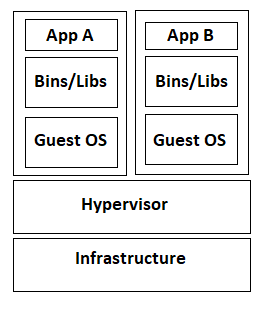
\includegraphics[width=0.5\textwidth]{Hypervisor.PNG}
  \caption[virtualization architecture]{virtualization architecture}
  \label{fig:virtualization architecture}
\end{figure}

\pagebreak Containerization, on the other hand, uses a different type of virtualization. In a containerization architecture there is no hypervisor, but a container engine which is situated on top of the operating system. This is beneficial as the operating system can no longer restrict certain applications from running. Containerization abstracts the underlying infrastructure by creating specific virtual pieces of the hardware infrastructure. This can be identified by image 2.2 below. The virtual aspects from the rest of the architecture are taken and create containers at the operating system level. When containerization is used, the operating system is the main feature and is shared among the containers. Whereas, in a virtualization architecture, the operating system is cloned for each virtual machine in the environment.

\begin{figure}[ht]
  \centering
      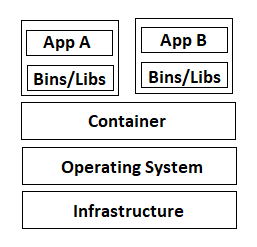
\includegraphics[width=0.5\textwidth]{Container.PNG}
  \caption[Containerization architecture]{Containerization architecture}
  \label{fig:Containerization architecture}
\end{figure}



\pagebreak As containerization essentially performs the virtualization of the operating system, this means that any type of compute device would be able to host a containerization platform. This is where single board computers come in. Single board computers as previously stated, are single circuit boards with microprocessors, memory, input/output and other aspects required to make a fully functioning computer.\cite{Reference17} There are many types of single board computers available if desired, throughout my time studying at Cork Institute of Technology I was exposed to two types of single board computers, Raspberry Pi's and Arduino's. A Raspberry Pi is a very popular single board computer which is used among schools and colleges to demonstrate how single board computers function. From figure 2.3 it can be seen that the Raspberry Pi is in fact a single switch board with all of the added commodities required by the user. One benefiting factor of this single board computer is the operating system element. A Raspberry Pi can a specialized Linux operating system, which, enables a user friendly environment.         


\begin{figure}[ht]
  \centering
      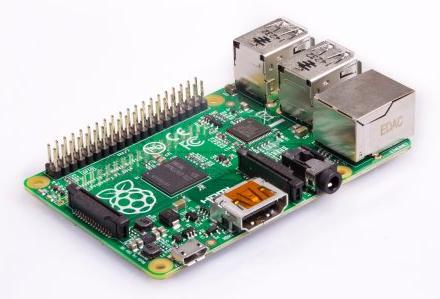
\includegraphics[width=0.7\textwidth]{RaspPi.PNG}
  \caption[RaspberryPi 2 Model]{RaspberryPi 2 Model \cite{Reference18}}
  \label{fig:RaspberryPi}
\end{figure}

\pagebreak The second single board computer which I will be researching for this project is an Arduino. Arduino is open-source, which is based off easy to use hardware and software. Arduino's function is by a micro-controller, this micro-controller can be sent any set of instructions that is to be executed. An Arduino can be used for a variety of things, depending on what the user desires. This element makes the Arduino appealing, but, Arduino's do not have their own operating system, meaning that the average user, with no programming knowledge would find it extremely difficult to benefit from the beauty of the Arduino.

\begin{figure}[ht]
  \centering
      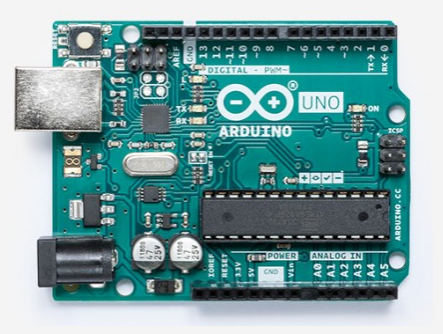
\includegraphics[width=0.7\textwidth]{Arduino.PNG}
  \caption[Arduino]{Arduino \cite{Reference19}}
  \label{fig:Arduino}
\end{figure}

\pagebreak Why single board computers? The decision to use single board computers throughout this project was adapted by a variety of reasons. They are inexpensive, open-source and easily usable. These aspects make this project achievable by anyone who would desire to re-create, while also helping to get the overall theory across as clearly and effectively as possible. These two types of single board computers are seen to be the most used in the world, meaning that users with any prior knowledge of computer science would know the functionality of these devices. For users who have no prior knowledge, the Raspberry Pi is a much more reactive single board computer. For this reason and for simplicity, two single board computers will be used throughout the implementation of this project. 

Single board computers are a necessity to achieve the desired outcome, but, the main reasoning behind choosing this topic was because of containerization. As containerization has been around for a long time but still quite unknown, I am going to delve into the area and outline every aspect of containerization.

\begin{itemize}
    \item What are containers?
    
    As previously stated containers are light weight software package that contains everything needed to run an application. More often than not, developers face issues when developing an application to ensure that it will be able to run on any device. To give an example of this, imagine having a mobile application, but it only being able to run on a Samsung phone but not an Apple device. Containers help to ensure that the application can be deployed anywhere. The functionality is, a container has a specialized environment which consists of all the underlying dependencies which would commonly be needed for development. On a higher level, libraries, binaries and configuration files (which can be seen from figure 2.2).
    
    \item Why containers?
    
    Containers are very lightweight, they can be only tens of megabytes in size in comparison to virtual machines. For this reason alone, containers are very appealing. Quick boot-up time is another huge benefit of containers. Having a quick boot-up time provides the application with almost instant run time, for instance, imagine having the option to have your laptop start-up and run straight away, or, needing to give it a few minutes to warm up before usage, having a quick start-up is always going to be the desired option. Finally, Containers and containerization, provides the opportunity to split all of the different aspects that an application would use to function into modules. This technique is also known as micro-services, another aspect of this project. Having the application split into modules allows for changes to be made much easier and conveniently, essentially, a developers dream. These modules can be installed and removed if required due to the light-weight architecture of containers.
    
    \item Types of containers
    
    The most popular container to date is Docker. Docker has single handily popularized container technologies over the last number of years. It has helped developers and corporations worldwide to understand that development and deployment can be made much simpler and more efficient. For this project, Docker is the container technology which I have chosen to be used as it is a Linux hosting container. But, there are many more container technologies that could be used. Tomcat, Jetty and Springboot are some examples of containers which are used by Java applications. Java containers are useful, but, Linux containers are going to be used for this specific project. Rocket containers or Rkt, was launched from CoreOS as a result of early security issues with Docker. These issues have been long been addresses, leaving Rkt behind. Even though there are these different types of containers, Docker is the one which is much more manageable.
    
    \item Docker
    
    Docker is an open-source container application which performs virtualization of the operating system in a virtual environment. It was designed and founded by Soloman Hykes, who is an engineer and now Chief Technology Officer of Docker. As previously stated, Docker is a Linux container but can also run on Windows OS and macOS. Dockers functionality is achieved by what are known as containers, these containers are run by a single operating system kernel ( a kernel is a computer program which controls every aspect of the system), which makes containerization much more lightweight than typical virtual machines.
    
    \item Managing Containers
    
    Like most things in technology, there is a level of management needed behind the scenes. Kubernetes is an open-source system for automating deployment , scaling and management of containerized applications. In other words, Kubernetes manages everything within a container. Kubernetes works extremely well with Docker, while Docker provides the container, Kubernetes orchestrates and manages the clusters of the container.  
    
    \item How does Kubernetes Work?
    
    Kubernetes is a platform for working with containers. It gives you the options to work with deployments, an easy way to scale and allows for monitoring. In Kubernetes, there is a master node which is used to create the container image you would prefer, this image then deploys and becomes the application. Kubernetes monitors of all of the applications which it has deployed, therefore, if an application were to go down, it tries to fix the issue and redeploy the application. In terms of scaling, Kubernetes will allow you to scale your application but will place the newly scaled deployment in a location which is determined by Kubernetes itself. This way, the resources are being used efficiently. 
    
\end{itemize}


%Position your topic within Computer Science. This activity will aid you in your literature review also. We zoom out to see three levels:

% notice the enumerate structure to create itemized lists
%\begin{enumerate}
   % \item What is the core topic your project is about? e.g., Mobile app for online voting. 
    %\item What core area(s) does the project fall under? e.g., Mobile applications, Social Networking, Service Providers. 
    %\item What main area(s) of Computer Science does the project fall under? e.g. Software Development, Cloud Computing.
%\end{enumerate}

%The ACM Computing Classification System (http://www.acm.org/about/class) will aid you in this, use the 2012 categories. Make sure to use figures and illustrations were appropriate. LaTeX will take care of the formatting of these. Do not try to get fancy here, you should concentrate on the content and not the formatting, this is why we are specifying LaTeX.

% Again take note of the structure, simply copy and paste this for future single figures


%You can specify the width and label for a figure which allows you to reference the figure and you can attribute a source in the figure caption as is done for figure \ref{fig:successkid}. Make sure you reference all external figures (i.e. figures you did not create yourself). Also use references for all figures e.g. use "... in figure \ref{fig:successkid} ..." NOT "... in the figure above ...".

%\section{Project Scope}
%Project specifics: Background minimum knowledge.

%Imagine you wanted to explain the specifics of your project to a person that knows nothing of Computer Science. You cannot talk about everything (as the idea is not to write a 500+ page report). Remember the reader at this stage can only be assumed to know what you have covered, so identify what are the minimum concepts belonging to the main areas (listed as 3 in the section before) and the core areas (listed as 2 in the section before) that you would need to explain so that the reader is able to understand the specifics of your project and indeed the following section. For example the minimum amount of knowledge about software development, cloud computing, mobile applications, social networking and service providers that are required so as to understand the specifics of a project about a mobile app for an on-line voting system. Here we are making the same trip we did before, but now in the opposite direction. Start zooming in from 3, then to 2 and finally to reach your project 1. Once the reader is finished this section they should be able to understand the proceeding sections (and have context for it within the project).


\section{A Review of Thematic Area}
During this section of the project, I will be displaying some of the resources that are available with regards to the topics I have and will be covering. Firstly, I will be discussing some of the conferences which are held all over the world on the topics of IOT, Cloud computing and containerization.

\begin{itemize}
    \item IEEE Global Conference on Internet of Things \cite{Reference2}
    
    IEEE stands for the Institute of Electrical and Electronics Engineers. This conference is held by the IEEE on the topic of Internet Of Things and its main goal is to provide a forum for innovation and research. This event is hosted annually at a range of different locations and provides keynote speakers from some of the top institutes in the world.
    
    \item Cloud Expo Europe \cite{Reference3}
    
    The Cloud Expo Europe conference dives into all aspects of cloud computing, including DevOps and infrastructure. As there are many aspects of cloud computing, this specific conference is divided up into specialized areas to ensure the attendies can get the full experience. These specialized ares include, Agile Networks, Fintech Finance and Banking Technology, Multi-Cloud strategy and management, and DevOps containers and open cloud. 
    
    \item KubeCon Europe \cite{Reference4}
    
    KubeCon Europe is run alongside KubeCon China and KubeCon North America. What makes KubeCon so appealing is that it focuses solely on Kubernetes and IOT, Micro-services and security for these aspects. It is also a Linux Foundation event which combines containerization and cloud computing communities together to hold open discussions. 
  
    
    \item DockerCon US and Europe \cite{Reference5}
    
    DockerCon is the most prestigious event of its kind. From its name, it is obvious who this conference is hosted by, Docker. Like other conferences, it offers a variety of panels with well known speakers and even workshops for its attendees. Anyone who uses docker or is interested in using docker attends this 3 day conference. 
    
    
    \item Cloud and DevOps World  \cite{Reference6}
    
    Cloud and DevOps world aims to delve into the world of cloud innovation. This includes containers and server-less architecture. It is a huge conference which is held in London annually and is hoping to change the future with cloud.
    
    
    
\end{itemize}


These conferences take place every year, proving that this area within computer science is very much relevant and constantly developing and improving. Along with these conferences, there are a number of books and journals written on the topics of Containerization, Single board computers and micro-services. 

\begin{itemize}
    \item \textit{Commodity single board computer cluster and their applications} \cite{Reference7}
    
    Commodity single board computer cluster and their applications is an article which is abstracted from volume 89 of the Future Generation Computer Systems journal. This journal covers all aspects of computer science and engineering. This article was released on the 30th of June 2018 and was written by a group of lecturers from universities around the United Kingdom. In short, this article dives into the area of single board computers specifically Raspberri Pi's along with the aspect of clustering SBC's. 
    
    \item \textit{Running Containers in Production} \cite{Reference8}
    
    This is a whitepaper which was released on the 19th of September 2018. The aim of this whitepaper is to explore the benefits of containers while also investigating the challenges that come with deploying containerized applications. The areas which are covered are building and managing container environments, monitoring and securing containers.
    
    \item \textit{The Docker Book} \cite{Reference9}
    
    Written by James Turnbull and released on the 4th of August 2014, The Docker Book containers everything one would need to know about the container Docker. Throughout this book, James writes in much detail about Docker along with every aspect that needs to be examined to understand containers and containerization applications.
    
\end{itemize}

There are many wikis, youtube videos and blogs regarding this area. I will list just some of these below:

\begin{itemize}
    \item Container Solutions \cite{Reference10}
    
    Container solutions is a blog which discusses all things container and containerization. Each blog post is written by a different individual who is an expert in this particular field. Container solutions has a huge following, with a newsletter emailed to those subscribed, there is no doubt container solutions will keep any individual up to date with all things containerization.
    
    \item Introduction to Micro-services, Docker and Kubernetes \cite{Reference11}
    
    This is a YouTube video which I found extremely helpful in the early stages of my research for this project. It explains in some detail the process of how Docker, Kubernetes and Micro-services coordinate and work together. The YouTube video was uploaded in November 2017 by James Quigley who has some videos regarding related topics. 
    
    \item Raspberry Pi Arduino Communication \cite{Reference12}
    
    Staying with YouTube videos, this video outlines how to connect Raspberry Pi's and Arduino's over a USB connection. This is extremely helpful to me as for this project, I will be attempting to migrate services between these two single board computers. The individual who is speaking explains in detail yet in a very understanding way the process of how to accomplish this communication. This YouTube video was uploaded by an account which is called nmBotTronics in January of 2016. 
    
    \item LoverPi \cite{Reference13}
    
    LoverPi is a website which is dedicated to all things Single board Computers. Not only is it a website which sells and distributes single board computers, but they also have a blog and wiki page dedicated solely to them. This is a one stop shop for everything related to SBC's.
    
    
    \item Degee U \cite{Reference14}
    
    Degee U is a YouTube channel run by DJ Spiess. DJ has been making videos on all topics related to programming, micro-services, Apache and many more for a number of years. One particular video which attracted me to his channel is his video titled "what are micro-services?". After watching this video I then found many other videos related to my topic of research from DJ and realized that his content would be of great use. 

    
\end{itemize}


As this project is based around the thematic area of Cloud Computing, HCI and Compute Systems, there are many companies worldwide who would design and implement what I hope to be the end product. Some of these companies include:

\begin{itemize}
    \item VMWare
    
    Is the leader in all things cloud infrastructure and virtual work-space technology. VMWare is known world wide for its ground breaking applications and infrastructure, their products are used by millions of customers in every corner of the world. 
    
    \item Google
    
    As a household name, every person to touch an online service has used Google's search engine. But, what many people who do not have the knowledge or an interest in the more in-depth aspect of this organization is, they have developed much more than just the Google search engine. Kubernetes was developed and founded by Joe Beda, Brendan Burns and Craig McLuckie. Once Google realized what Kubernetes was going to be, they sent two more engineers to ensure the application would be designed to its best ability. These two men were Brian Grant and Tim Hockin.
    
    \item Docker 
    
    Docker, as previously stated, is a container application which performs the virtualization of the operating system in a virtual environment. How Docker is going to be used in this project is unique as I will be installing Docker on single board computers, whereas Docker would typically be installed on much larger devices. 
    
\end{itemize}

%The focus of this section is at the heart of the project research phase. You must identify the main sources of information you should be aware of within your chosen area and pay regular attention to so as to strengthen your knowledge in the core topic you are working at. So here you should develop an knowledge of not only your core topic but also about the area of computer science the topic falls under. More specifically you should research the following:
%\begin{itemize}
   % \item The top 5 International Conferences and Journals most related to your topic. This is crucial, as it represents the main source for keeping you aware of what the state-of-the-art in your topic is.
  %  \begin{itemize}
        %\item In particular it will make you aware of what other projects related to yours have been already done (so that you can compare/position your project w.r.t. these).
        %\item What new techniques are being developed, so that you can apply them in your work. e.g. new frameworks for data visualization
  %  \end{itemize}
    %\item The top 3 most recent books/texts related to your topic. There are many free resources from which you may download a relevant text on the topic of your project. Try to either download or borrow 3 recent (no older than 10 years) texts relating to the topic your project is on which you will use throughout the project as reference material and to aid in tackling a number of the technical problems you may encounter. Any PhD/MSc thesis that have published in the last 5 years relating to the topic are also invaluable resources as they will contain a state of the art and references in your project topic. Approach these only after reading/viewing the wikis/Youtube videos you find as a certain level of knowledge will be assumed about the topic.
    %\item The top 5 companies/organizations potentially interested in the product you are developing. Finally, this is also crucial, as it forces you extend to purely programmer view of the project to a wider view considering the market, potential stakeholders and niches where your product can become useful. Moreover, Computer Science is a huge topic with loads of different works and roles. If you pick a project in the area you feel passionate about, and you identify what the market in this area is about, then you can drive your future professional career (from the very beginning) towards the path that makes you happier. I know that this does sound as a very technical reason, but I suppose we all agree is probably the most important of all reasons for choosing a particular project focus. 
    %\item The top 5 wiki/forums/blogs/Youtube channels most related to your topic. This is crucial to you as well, as it represents a more accessible, personal and less informal way of communication with people working/interested on the same topic as you are. This communication is extremely helpful for improving your skills, solving potential doubts and increase the interest/relevance of the topic/area itself.
%\end{itemize}

%You should begin your journey of discovery in reverse order to the listing above (which is given in order of academic importance/significance). So when you are researching your topic first look up some TedX talks or youtube tutorials, then research what companies are doing in the area, then get a handful of very good texts on the core topics of your area (anything older than 5 years usually is not helpful here) and finally start reading conference or journal papers (again newer is better here). In particular during this section you may need to use tables to list resources. These are also automatically formatted in latex thus allowing you to concentrate on content. for example table \ref{tab:Mylar}.

%\begin{table}[ht]
	%\centering
		%\begin{tabular}{ c  c  }
	%	\hline
	%	\hline
	%	Parameter & PET \\
	%	\hline
	%	Youngs Modulus & 2800-3100MPa \\
	%	Tensile Strength & 55-75MPa \\
	%	Glass Temperature & 75$^\circ$C \\
	%	Density & 1400kg/m$^3$ \\
	%	Thermal Conductivity & 0.15-0.24Wm$^{-1}$K$^{-1}$ \\
	%	Linear Expansion Coefficient & $7\times10^-5$ \\
	%	Relative Dielectric Constant @ 1MHz & 3\\
	%	Dielectric Breakdown Strength & 17kVmm$^{-1}$\\
	%	\end{tabular}
	%\caption{PET Physical Properties}
	%\label{tab:Mylar}
%\end{table}

To this current day, there has been much work performed in all of the areas this project falls under. One area in particular which has grown substantially in the last 10 years is Cloud Computing. When the term cloud computing first emerged back in the 2000's, people were confused as to what exactly it was. Now, the cloud is used in many ways and can be tailed to a specific need. In short, cloud computing can benefit organizations by minimizing their IT infrastructure costs. One main aspect of cloud computing is virtualization. Virtualization aims to speed up the operations in an organization while reducing costs, this is achieved by splitting physical components of a computing device into several virtual devices. These virtual devices can be easily managed and scaled, which is a characteristic that can be very appealing to growing corporations. There are many types of cloud computing or services available to its users.

\begin{itemize}
    \item \textit{Infrastructure as a Service (IaaS)}
    
    This service provides resources over the internet in a virtual manner. This model allows the cloud provider to host the fundamental assets of the infrastructure in an on-premise data centre. This allows for easier, faster and most importantly, a more cost effective operation of the underlying infrastructure. IaaS typically uses a management or orchestration technique to ensure that the virtual environment is run efficiently and to the highest standard.
    
    
    \item \textit{Platform as a Service (PaaS)}
    
    Platform as a service allows customers to manage, develop and run applications with ease. These customers would no longer be forced to worry about building complex infrastructures to develop and run such applications. Typically, this infrastructure is provided by a third party company who would allow access over the internet to such service. This is beneficial as having an underlying platform, which could include both hardware and software, to develop and run applications can be extremely costly. This cost is cut substantially if Platform as a service is implemented. A PaaS provider would analyze the situation and implement what they think is needed to ensure a business can perfrom the tasks required. 
    
    
    \item \textit{Software as a Service (SaaS)}
    
    SaaS provides the essential software that organizations would require. Third party companies provide applications to their customers over the internet. Usually, this would be at a fixed cost. For example, Cork Institute of Technology uses Gmail to host all of the email accounts for students and staff, this is a service which is provided over the internet to CIT. As a result, this removes the obligation of CIT to install a server to run this application, again, cutting costs. The ability to scale is a huge benefit of SaaS, again taking the email example from CIT, as more student enroll each year, more email addresses can be provided with much ease. 
    
\end{itemize}

Computing and Computer Science is changing rapidly, with new technologies being launched quicker than ever before. It is important to keep informed of these new trends and technologies. Two new technologies which have emerged recently are Edge Computing and Fog Computing. These technologies aim to ensure that the compute technologies involved in a network are functioning to the highest possible standard. This is achieved by working together and  pushing the huge amounts of data which is generated by IOT devices to different platforms which are one the edge of the network. 

\begin{itemize}
    \item Edge Computing
    
    Edge computing is exactly as it sounds. IOT devices can be referred to as edge devices. As we already know, single board computers are IOT devices as they generate their own data. Edge computing maintains all the data which was generated on it, while staying on the edge of the network. This is beneficial as it can help keep the network secure. 
    
    \item Fog Computing
    
    Fog computing is an architecture which is designed to connect cloud computing to the edge. Also referred to as the missing link in connecting and sending data to the cloud environment. Fog computing can be used to reduce bandwidth needed within network, as the devices are directly connected and data does not need to be sent back and forth between data centres. 
    
    
\end{itemize}

With the type of environment that will be created using single board computers to migrate micro-services, this could be considered a small fog/edge computing network. 

Complex Systems and Internet of Things are two areas which can be interlinked. There are studies which have occurred from many Universities on the topic of how IOT can help in managing complex systems. But what exactly is the Internet of Things? 

\begin{itemize}
    \item Internet of Things 
    
    The term internet of things evolved from Massachusetts Institute of Technology (MIT) in the late 1990's. Essentially, IOT is any device which can be interconnected. How these devices are connected comes from their ability to connect to the internet. Not only are these devices interconnected but they also collect and exchange data. Examples of IOT include, smart watches, smart phones and sensors, the list is endless and with new IOT devices being developed everyday, eventually everything will be classed as an IOT device. More recently, IOT devices allow freedom to its owners by acquiring the ability to be monitored and controlled from a remote location. Single board computers are classes as IOT devices as they can be interconnected and also have the ability to be connected to the internet and provide such data. 
    Data that is collected from IOT devices is being analyzed and examined by the creators. Like anything that is connected to the internet, data is generated and can be analyzed for research, used by businesses for analytics and/or to form a profile of you as a user. Some companies use this data to figure out what their next big strategic step would be.
\end{itemize}


%What has been done before in your community w.r.t. your topic? Once you have gotten an understanding of the topic and technologies and have identified the top 5 formal conferences/journals, wiki/forums/blogs/Youtube channels and companies/organizations the next step is to research in depth on them! And here in depth means in depth. Make sure you cite\cite{Reference1} a number of papers \cite{Reference3}, luckily Latex will take care of the ordering of the citations \cite{Reference2} for you.

%The aim here is that you find the trends in your topic (3), and more in general in the area in which your topic resides (2) your project falls under and from these trends you develop your initial project question further and begin to get insights into how others have solved/approached similar problems. Think of this section as colouring in your initial idea. Before you approach this section you should read at least 4/5 good literature reviews (a selection of last years projects will be posted on blackboard to aid you but you should find other sources also).

%In particular in this section, you must find and analyze at least 5 (ideally around 10) works belonging to, or at least related to, your work. You must describe these works and position your project w.r.t. them (i.e., clearly identify the similarities and differences between your project and each of these works). Also remember if you find that you are detailing topics that you have not introduced already here you need to add something to the earlier Scope section. % Background Theory 


\chapter{Problem - Migrating Micro-Services between Single Board Computers using 
Containerization }
\label{chap:problem}
\lhead{\emph{Problem Statement}}
%The key question to be addressed in this chapter is: "What do I want to achieve".
%This chapter should comprise around 1500 words and describe the problem you are trying to solve. Try to be as specific here as you can, this will help you to anticipate possible risks such as lack of support from APIs.

\section{Problem Definition}
While progressing through this project, I am going to be delving into all aspects of containerization, single board computers, edge/fog computing and migration. As already established, the idea for this particular project is to investigate if micro-services can be migrated between single board computers using containers. Containers are widely used in many aspects of computing, but, there are very little studies on containers being placed on single board computers. Because there is very little regarding this topic, I decided to take it upon myself to investigate such aspect. By placing containers on single board computers, and proceeding to try migrate some micro-services between two single board computers. As previously discussed, the aim of containers is to allow software and/or applications to run on any compute system. This is necessary for many reasons. One main constraint developers face when designing new applications and services involves the physical compute system they are lying on. Different brands of devices have a variety of specifications which need to be met by these developers. Containers provide an additional platform layer between the operating system of a device and the applications which usually would be situated on-top. Having this additional layer is what allows any applications to run on the operating system. For example, if an application was developed for a Mac iOS device, it would have the underlying API's which are specifically designed for a Mac operating system, preventing this application to run on a windows device. To prevent this from occurring, a container could be placed on the windows machine, allowing the application to run exactly as it would on an Apple Mac device. 

%Describe the problem you are trying to solve in this project. There will sometimes be a need at some point during the report to display an equation that may be core to your project. For example if the project is on gait detection what equation are you using to determine gait? If the project is on localization what is the method/formula? The formatting of these is reliably done in Latex also as we can see in equation \ref{eq:Legrange}.


\section{Objectives}
The main objective of this project is to migrate micro-services between two Raspberry Pi's. Managing micro-services requires a specialized program which will lie on the container. The management application provides a level of orchestration for these micro-services. Kubernetes is the orchestration tool which will be used for this project. Kubernetes prides itself in being an open-source orchestration tool for containers. The reason which Kubernetes is used when managing containers falls under the issue of connecting these containers to the outside world. Kubernetes provides scheduling, load balancing and distribution which are essential elements in any device. Kubernetes aims to ensure containers run exactly how a user intends. While all of this occurs, I will be investigating if this type of architecture falls under the category of edge or fog computing. The main reasoning behind this is to investigate whether single board computers and containers can be used in a fog environment and how beneficial it may be. 
%Enumerate the objectives you want to achieve in your project. Again as this is an early stage these will tend to change but there should be a rational explanation for this change. Always document your work, keep a lab book during the term that you only use for FYP!

\section{ Requirements}
For this project to be achieved, there are many requirements which are essential. These are as follows:

\begin{itemize}
    \item Single Board Computers
    
    A Raspberry Pi is a requirement for this assignment this is where the functionality will be held. For this project to be successful there is a compute system needed. A raspberry Pi is a compute device which is portable, light-weight and affordable and can be scalable if necessary.
    
    \item Containers
    
    As previously discussed, containers allow developers a more functional way to develop and deploy applications. Using containers to host micro-services allows applications to run on any device regardless of the underlying operating system. The container of choice for the project as stated is Docker.
    
    \item Container Orchestration Tool
    
    With containers, an orchestration tool is needed to ensure they are functioning to their full ability. Kubernetes is an application which provides this level of orchestration which is needed.
    
    \item Micro-services
    
    Micro-services lie within a container. As mentioned, micro-services are beneficial as they are easily deployed, scalable and work effectively in with containers. 
    
\end{itemize}


%Enumerate the functional requirements you want your project to have. 

%Please, do not include the use cases here. If you want to create a one-to-one mapping between functional requirements and use cases (which does not necessarily need to be the case, indeed most likely this will not be the case) do it elsewhere. Here should purely describe what do you want to do. In no case should you use this section to provide a description of how to implement them, that is for later. For people doing projects that are not heavy implementation projects (e.g. deploying an architecture or testing a novel tool in specific conditions) this structure can still be used as it will force you to think about what you plan to achieve and what possible metrics you may need to measure success.

%Let me explain this with more detail. A common mistake is that people confuse the problem description with the solution approach. This is a common mistake by confusing the \emph{what} with the \emph{how}. Here we are purely focused on the what: What is this project about? What are the objectives? What are the functional and non-functional requirements? 

%How are we going to do all these things? Well, this is a question for next chapter. Provided a problem, an objective or a functional requirement, obviously there will usually be many ways of doing it, thus there will be many \emph{hows}, but the definition, the \emph{what} we want to achieve will be unique.

%One other display structure you may wish to use at some stage during the report is a figure array. This can also be easily done with Latex and is shown in figure \\%ref{fig:twosuccesskid}

%\begin{figure}
%\centering     %%% not \center
%\subfigure[Figure A]{\label{fig:a}\includegraphics[width=0.48\textwidth]{successkid.jpg}}
%\subfigure[Figure B]{\label{fig:b}\includegraphics[width=0.48\textwidth]{successkid.jpg}}
%\caption{Two Success kids}
%\label{fig:twosuccesskid}
%\end{figure}



 % Problem

\chapter{Implementation Approach}
\label{chap:implementation}
\lhead{\emph{Implementation Approach}}
%The key question to be addressed in this chapter is: "How do I plan to achieve what I have outlined in the previous chapter".

%This chapter should comprise around 5000 words and specify your planned implementation approach. Again all sections below are suggestions and will vary significantly from project to project, the key element to be addressed is the core question of the chapter.

%\section{Architecture} \label{sec:Arch}
%Describe the architecture of the solution that you have in mind, including:
%\begin{itemize}
  %  \item Technologies involved (e.g., frameworks, programming language). 
 %   \item The hardware needed to develop the project (and to support at deployment stage)
%\end{itemize}

%Provide a high level view of the system you have in mind, including any package of classes, what is it responsible for and what other packages it communicates to. Provide a high level view of the database (or structure) needed to support the project, including what each table/document is responsible for and the hierarchy among them. You need to be as specific here as you can, why? Because this will aid you in identifying parts of the project you are vague on, this may be fine for some components but cause problems in term 2 for others. If you have hardware element in your project this is also where you provide a high level view of how these elements integrate into the project. So for a project that is cyber-physical you will have both a hardware and software architectural diagram. N.B. This is NOT a full system design but a high level overview of what you can credibly develop. This architecture should be informed by prototyping activity. 

%Some of the implementation focused projects may describe how do you envision tackling the functional requirements of your project via a set of use-cases. DFDs are also helpful here to understand elements of your project that may cause problems. You should describe the role of the different parts of the architecture of the solution, and the interaction among them.

\section{Risk Assessment}
With every project comes a risk. A risk is the possibility of losing something of value, an intentional interaction which can cause uncertainty. In any project there is a possibility that when progressing through the plan, that it becomes clear there is no feasible way the project can be implemented. This is also a possibility when implementing this idea. The technologies which are being used have been widely explored, proving their functionality. But there are no studies which show the migration of micro-services between devices. Although this is the case, there is no reason any issue which may rise can not be worked around or fixed. But, to be sure a risk analysis assessment must be carried out:

\textbf{ \underline {Uncertainty}} - \textit{Moderate}

Uncertainty is defined as an area of increased risk within a project. The level of uncertainty here is moderate. There are elements which are known to be fully functional, for example, we know that Raspberry Pi's are fully functioning single board computers. But, there is also the risk that the container might not sit correctly on the Raspberry Pi, which could lead to a whole re-work of this theory.

\textbf{\underline{Complexity}} - \textit{High}

Both complexity and uncertainty can be closely linked. Complexity aims to identify the level of difficulty attached to a project. For this project, the level of uncertainty is high. The reasoning for this is again, this is a new technique which has very little exploration, therefore, leaving the implementation to be widely unknown.

\pagebreak
\textbf{\underline{Size}} - \textit{Moderate}

The size and scale of a project is important to consider. The size of this project is moderate, the good thing about having this project implemented on Raspberry Pi's is scalability is never an issue. These edge devices can be moved, added and removed with little effort. Therefore, size would not be much of a risk factor. For this project, using just two SBC's keeps an element of simplicity.


\textbf{\underline{Project Management Level}} - \textit{High}

Project Management is extremely important. Project management involves planning, controlling and executing the tasks which are set out at the beginning of the project plan and ensure each stage is achieved as desired. 



%hese technologies, which enforces the possibility of failure.IFrom my research, there is very little to display that this would be a failure. The technologies are extremely scalable and flexible, which is exactly what is needed.dening ttify any potential risk precluding you from successfully complete your project. This section is really important and often neglected by students resulting in fatal risks occurring in some projects. Make sure to give this section the time it requires. Classify the risk according to their importance, possibility of arising and enumerate the decisions you can make to anticipate them or mitigate them (in case they finally arise). Table \ref{tab:ProjRisks} may help with this classification. This section should include your mitigation approach for any critical risks.

%\begin{table}[h]
%\centering
%\scriptsize
%\caption{Initial risk matrix}
%\begin{tabular}{|p{2cm}|p{2cm}|p{2cm}| p{2cm} |p{2cm}| p{2cm}|}
%\hline \bf Frequency/ Consequence & \bf 1-Rare & \bf 2-Remote & \bf 3-Occasional & \bf 4-Probable & \bf 5-Frequent\\ [10pt]

%\hline \bf 4-Fatal & \cellcolor{yellow!50} & \cellcolor{red!50} & %\cellcolor{red!50} & \cellcolor{red!50} &\cellcolor{red!50} \\ [10pt]

%\hline \bf 3-Critical &\cellcolor{green!50} & \cellcolor{yellow!50} & \cellcolor{yellow!50} & \cellcolor{red!50} &\cellcolor{red!50} \\ [10pt]

%\hline \bf 2-Major & \cellcolor{green!50} & \cellcolor{green!50} & \cellcolor{yellow!50} &\cellcolor{yellow!50} &\cellcolor{red!50} \\ [10pt]

%\hline \bf 1-Minor & \cellcolor{green!50} & \cellcolor{green!50} & \cellcolor{green!50} &\cellcolor{yellow!50} &\cellcolor{yellow!50} \\ %[10pt]
%\hline
%\end{tabular} \\
%\label{tab:ProjRisks}
%\end{table}

\section{Methodology}
%Describe your personal approach on how to tackle the different parts of this project, including:
%\begin{itemize}
 %   \item How to tackle the needed research to fulfill the background chapter. 
  %  \item How to set up your Computer Science skills to the project needs (e.g., describe your plan to learn any new technology involved on the project that you are not familiar with). 
   % \item What core project managing approach will you follow (e.g., Waterfall, Scrum, etc).
%\end{itemize}

There are many elements, needed to bring this idea to reality. One element which is hugely important and is the backbone for any project is the research. To ensure accurate and efficient information is provided, extensive research must be carried out. For the research of this project, it was important that all information was sourced from a variety of sources. These included books, ebooks, journals, wikis, blogs and whitepapers. 

The background research is needed to ensure this project will come together, but, as this is a project based on computer science subjects and technologies, there is more in-depth learning required. From the hardware to the software which will be used, there is some level of upskilling needed. This includes:

\textit{Raspberry Pi}

Learning the setup and functionality of a Raspberry Pi. This is a very important step as the Raspberry Pi backbone of this project. Setting up the SBC's is going to be the first step in the implementation phase. Because of this, knowing every aspect and detail required to ensure that this technology can be used to its highest potential for this project is essential. There are many many books and tutorials online to help with this process, which have been and will continue to be hugely beneficial throughout the implementation phase. 

\textit{Containers}

Containers are what this project is mainly focused on. Meaning, that extensive research needs to be taken on this element. As containers are a somewhat unknown technology and is not explored in my chosen course of study, the research and learning curve has been taken upon myself solely for this. With much information on containers and different types of containers and container orchestration tools, this element of the project will be an interesting and exciting one. 


Most of the other technologies involved are ones which have been studied over the last four years of studies in Cork Institute of Technology. Even though this is the case, due to any potential risk that could occur, it is important that research is continually carried out throughout both the research and implementation phases. This is mainly to ensure the project idea can be delivered to the highest ability. 


Every project requires management. For this project I researched some project life-cycle models to decide which would best be suited to this particular project. There are many life-cycle models which can be implemented for projects of this type. These include \textit{waterfall}, which is the oldest type of life-cycle used, it includes setting phases and not moving onto the next phase until the phase before is completely finished. Next, \textit{Agile}. This type of project life-cycle focuses on mainly software development, but can be used by project managers for all technology type of projects. The aim of the agile method is for the project manager to continually inspect and asses the workings of the team to ensure sufficient work and goals are being achieved. And finally, \textit{evolutionary} model. The evolutionary model is split into two main models, spiral and prototyping. The spiral model works alongside the prototyping model to mainly asses the risk which is attached to the different stages of the process. The prototyping model's main focus is to produce a fully functioning prototype for the project at hand. 

\vspace{5mm}
\textbf{\large Evolutionary Model}

The life-cycle model which is appropriate for this project is the evolutionary model. As previously discussed, this model can be used for projects which have a prototype aspect while also assessing the risks which are inevitable in a project. This project is heavily focused on developing a prototype. The evolutionary prototype model has five phases which work towards quick development of the prototype required. As seen in figure 4.1, these phases include communication, quick design, modeling quick design, construction of prototype and deployment, delivery and feedback.



\begin{figure}[ht]
    \centering
      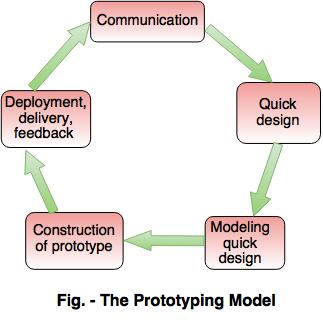
\includegraphics[width=0.65\textwidth]{Figures/PrototypeModel.jpg}
  \caption[prototype model]{Evolutionary Prototype Model \cite{Reference19}}
  \label{fig:Prototype Model}
\end{figure}

\vspace{5mm}

\begin{figure}
    \centering
     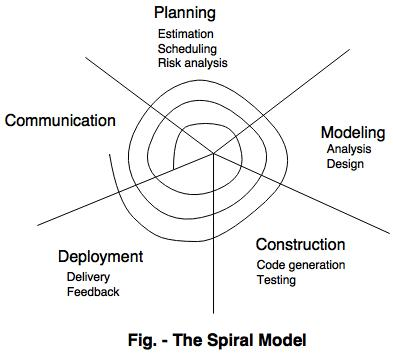
\includegraphics[width=0.65\textwidth]{Figures/SpiralModel.jpg}
  \caption[spiral model]{Evolutionary Spiral Model \cite{Reference19}}
 \label{fig:Spiral Model}
\end{figure}

\pagebreak

Not only are these phases used for the prototyping model, but they are also used for the spiral aspect of the evolutionary model. As seen in figure 4.2, the same phases are used to asses the risks which could potentially occur. 


\section{Implementation Plan Schedule}
%Come up with a schedule for the remaining time (including second semester), so as to describe how do you envision to achieve the implementation of your project by the end of semester 2. This plan SHOULD be ambitious but MUST be realistic and SHOULD be informed by early prototyping and MUST be discussed with your term 1 supervisor.

Throughout the implementation phase of this project, there will be a total of 200 hours expected to be invested. This level of commitment is needed for a project of this stature as there is a lot of additional research needed throughout. As seen from the risk assessment, there is a level of uncertainty involved with this project. I will break down the plan and time-line for the second phase of the project in a table:

\vspace{5mm}
\begin{tabular}{ |p{1cm}|p{6cm}| }
 \hline
 \multicolumn{2}{|c|}{Implementation Plan} \\
 \hline
 Week & Plan\\
 \hline
 1   & Install Operating System's on both Raspberry Pi's \\
 \hline
 2  &  Install Containers (Docker) on both Raspberry Pi's\\
 \hline
 3 & Troubleshoot any issues which may rise during installation process\\
 \hline
 4 & Install Kubernetes on both Containers\\
 \hline
 5 & Troubleshoot and resolve any issues which involve Kubernetes\\
 \hline
 6 & Install Virtual Machines on Kubernetes as Micro-services\\
 \hline
 7 & Test Virtual Machines and troubleshoot any issues\\
 \hline
 8 & Attempt migrating of microservices from one RP to the other \\
 \hline
 9 & Investigate and Troubleshoot issues which may occur. \\
 \hline
 10 & Investigate the aspect of transforming topology into an edge/fog environment \\
 \hline
 11 & Attempt to implement this type of architecture \\
 \hline
 12 & Review and Document all workings\\
\hline
\end{tabular}

\pagebreak
Having 12 weeks to implement the project in the second semester, I have set a goal of having one task to complete a week. These tasks are set with the mind set that they will take an estimated average of 16 hours each. 16 hours is a lot of time to allocate per week/per task but, from the research carried out in this phase of the project, it is clear every hour will be used to full advantage. Below is image 4.[], a Gantt chart of the estimated times I expect each task to take: 
\vspace{8mm}

\begin{figure}[ht]
    \centering
     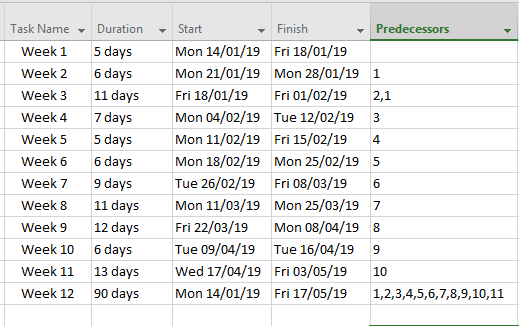
\includegraphics[width=0.95\textwidth]{Figures/ProjectPlan.PNG}
  \caption[Gantt chart Times]{Gantt Chart Times \cite{Reference19}}
 \label{fig:Gantt chart Times}
\end{figure}

\vspace{10mm}

Some of the tasks above can be seen to have shorter duration's than others. The reasoning behind this is to allow for some extra time to troubleshoot issues which may occur and potentially make any changes needed to improve the fore-coming prototype. Figure 4.4 shows the gantt chart layout for this project and how time will be spent during the implementation phase or second semester of this project. From January to May there is one continuous linked task which is set to write the required documentation for the implementation phase while ensuring weekly that tasks are being achieved. 
\pagebreak

\begin{figure}[ht]
    \centering
     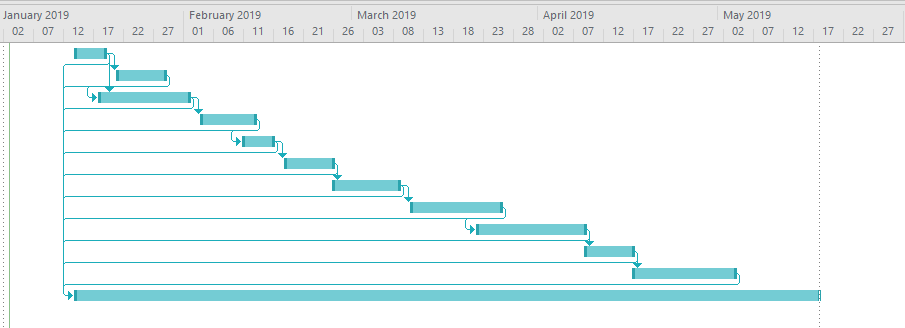
\includegraphics[width=1.0\textwidth, height=10cm]{Figures/GanttChart.PNG}
  \caption[Gantt Chart]{Gantt Chart \cite{Reference19}}
 \label{fig: Gantt Chart}
\end{figure}


\section{Evaluation}
%Come up with an evaluation plan that allows you to measure how much have you actually achieved the goals of your project. This again is a section that is often neglected where students loose marks. How do you plan to measure the output of your project? A binary it works/does not work is insufficient. You need to be able to quantify the success against both the functional requirements and the initial idea. These are not the same as you may meet all function requirements outlined but not solve the overall problem because you have failed to revisit these and update them with new information which you learn as you are developing the project.
Evaluating is essential to ensure that an accurate examination of the project is taken. The main aim of an evaluation is to analyze all aspects while assessing the outcome of the project. To achieve an effective project in both research and implementation, it is important to ask important questions:

\begin{enumerate}
    \item What was the purpose of the project?
    \item What is the expected outcome of this project?
    \item Who will this project benefit and why?
    \item Will this project be of use in future technologies?
    \item Are project targets being met and will they continue to be achieved?
    \item How will the project be assessed to ensure requirements are being met? 
\end{enumerate}

These being just some important questions which need to be answered. Project managers should gather information from an evaluation and use this information to determine the route to which the project takes. For this project, the evaluation would be based around the practicality of the migration of micro-services. The following questions need to be completed throughout this evaluation both before the implementation and during:

\begin{enumerate}
    \item Does the chosen container function on the Raspberry Pi?
    \item Will kubernetes run effectively on this container?
    \item Is it possible to install virtual machines on kubernetes?
    \item Will the migration of these micro-services be feasible?
    \item How will issues be resolved which may occur?
    \item Is it possible to share data other than microservices between the two Raspberry Pi's?
\end{enumerate}

Once these questions are repeatedly asked and answered throughout the course of the project, then understanding where the project direction is going will be much more clear. 

\section{Prototype}
%Although you do not have a fully functional project yet, you should show wireframes, snapshots or representation on how do you envision your project to look once the implementation phase has been completed. The nature of this section will vary significantly from project to project and can include anything from code snippets to snapshots of service deployments. Any prototyping you have done during the term should be summarized here that has not been captured in earlier sections. For example if you are planning to host your project using AWS in an EC2 instance you should have at least created a "hello world" setup to determine the basics, this probably should have been discussed in section \ref{sec:Arch}.
During the implementation phase of this project, I will aim to design a functioning prototype. This prototype will consist of the following aspects:
\begin{itemize}
    \item Two Raspberry Pi's
    
    These raspberry pi's will be used as the core compute systems. 
    
    \item Docker
    
    Docker, the container element of this project, will be installed and ran on the raspberry pi's. Here is where all functionality will occur.
    
    \item Kubernetes
    
    The orchestration tool for the containers, providing an overall view of the system.
    
    \item Virtual Machine
    
   Raspberry Pi's can be configured to have a Linux operating system to function. A virtual machine or machines, will be installed on the Raspberry Pi to show the functionality of micro-services.  
    
\end{itemize}

\pagebreak
As a general overview, figure 4.5 outlines the basic layers of this project:

\begin{figure}[ht]
    \centering
     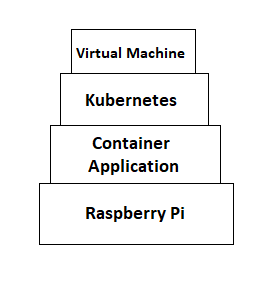
\includegraphics[width=0.45\textwidth, height=8cm]{Figures/Architecture.PNG}
  \caption[Architecture Layers]{Architecture Layers \cite{Reference19}}
 \label{fig:Architecture Layers}
\end{figure}

The prototype for this project will take some time to develop, as seen in the evaluation section. The final product will have the appearance of just two raspberry Pi's connected to a keyboard, mouse and monitor. From the outside appearing to be quite a simplistic prototype, the core of the raspberry pi's is where the technology lies to perform the function set out. 

The two Raspberry Pi's will be connected to a keyboard, mouse and monitor as shown:


\begin{figure}[ht]
    \centering
     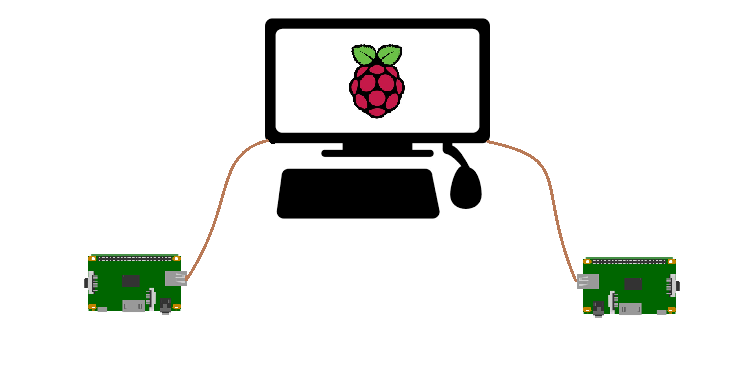
\includegraphics[width=1.0\textwidth,  height=8cm]{Figures/Topo.PNG}
  \caption[Topology]{Topology \cite{Reference19}}
 \label{fig:Topology}
\end{figure}


Once the Raspberry Pi's have been connected to a monitor, keyboard and mouse, each will be configured with an operating system. Raspbian is the operating system which the Raspb

Each Raspberry Pi will be configured with Docker. As previously discussed, Docker is the container engine being used for this project. Once Dock % Solution Approach

\input{Chapters/Chapter5} % Conclusions and Term 2 work

%% ----------------------------------------------------------------
\label{Bibliography}
\bibliographystyle{IEEEtranN}  % Use the "IEEE Transaction" BibTeX style for formatting the Bibliography
\bibliography{Bibliography}  % The references (bibliography) information are stored in the file named "Bibliography.bib"
\lhead{\emph{Bibliography}}  % Change the left side page header to "Bibliography"

%% ----------------------------------------------------------------
% Now begin the Appendices, including them as separate files

\addtocontents{toc}{\vspace{2em}} % Add a gap in the Contents, for aesthetics

\appendix % Cue to tell LaTeX that the following 'chapters' are Appendices

\input{Appendices/AppendixA}	% Appendix Title

\input{Appendices/AppendixB} % Appendix Title

%\input{Appendices/AppendixC} % Appendix Title

\addtocontents{toc}{\vspace{2em}}  % Add a gap in the Contents, for aesthetics
\backmatter
\end{document}  % The End
%% ----------------------------------------------------------------